% ╔══════════════════════════════════════════════════════════════════╗
% ║  Саморазвивающийся поток: архитектура обучающейся системы       ║
% ║  Компилировать: xelatex self_evolving_flow.tex                  ║
% ╚══════════════════════════════════════════════════════════════════╝

\documentclass[12pt, a4paper, twoside]{article}

% ─── Шрифты и язык ───────────────────────────────────────────────
\usepackage{fontspec}
\usepackage{polyglossia}
\setdefaultlanguage{russian}
\setotherlanguage{english}
\setmainfont{Liberation Serif}
\setsansfont{Liberation Sans}
\setmonofont[Scale=0.85]{DejaVu Sans Mono}

% ─── Геометрия страницы ──────────────────────────────────────────
\usepackage[
  a4paper,
  top=25mm,
  bottom=25mm,
  left=30mm,
  right=25mm,
  headheight=25pt
]{geometry}

% ─── Базовые пакеты ──────────────────────────────────────────────
\usepackage[protrusion=false,expansion=false]{microtype}
\usepackage{setspace}
\usepackage{parskip}
\usepackage{booktabs}
\usepackage{longtable}
\usepackage{array}
\usepackage{enumitem}
\usepackage{graphicx}
\usepackage{float}
\usepackage{caption}
\usepackage{subcaption}
\usepackage{amsmath}
\usepackage{amssymb}

% ─── Цвета ───────────────────────────────────────────────────────
\usepackage[dvipsnames, svgnames, x11names]{xcolor}
\definecolor{AccentBlue}{RGB}{25, 90, 160}
\definecolor{AccentTeal}{RGB}{0, 120, 120}
\definecolor{AccentOrange}{RGB}{200, 80, 0}
\definecolor{LightGray}{RGB}{248, 248, 250}
\definecolor{MidGray}{RGB}{130, 130, 140}
\definecolor{DarkGray}{RGB}{40, 40, 50}
\definecolor{CodeBg}{RGB}{245, 246, 250}
\definecolor{CodeBorder}{RGB}{200, 205, 220}
\definecolor{RuleColor}{RGB}{25, 90, 160}
\definecolor{LinkColor}{RGB}{10, 80, 160}
\definecolor{GreenOk}{RGB}{30, 140, 60}

% ─── Гиперссылки ─────────────────────────────────────────────────
\usepackage[
  unicode,
  colorlinks=true,
  linkcolor=LinkColor,
  urlcolor=AccentTeal,
  citecolor=AccentOrange,
  pdftitle={Саморазвивающийся поток: архитектура обучающейся системы},
  pdfauthor={Opus Research},
  pdfsubject={development\_system :: Common Lisp :: LLM},
  pdfkeywords={Common Lisp, LLM, саморазвитие, агенты, memory}
]{hyperref}

% ─── Код (listings) ──────────────────────────────────────────────
\usepackage{listings}
\usepackage{lstfiracode}  % опционально; если нет — fallback
\lstset{
  basicstyle=\small\ttfamily\color{DarkGray},
  backgroundcolor=\color{CodeBg},
  frame=single,
  framerule=0.6pt,
  rulecolor=\color{CodeBorder},
  breaklines=true,
  breakatwhitespace=false,
  showspaces=false,
  showstringspaces=false,
  showtabs=false,
  tabsize=2,
  captionpos=b,
  numbers=left,
  numberstyle=\tiny\color{MidGray},
  numbersep=8pt,
  xleftmargin=14pt,
  xrightmargin=4pt,
  aboveskip=10pt,
  belowskip=6pt,
  escapeinside={(*@}{@*)},
  literate=
    {а}{{\cyra}}1  {б}{{\cyrb}}1  {в}{{\cyrv}}1  {г}{{\cyrg}}1
    {д}{{\cyrd}}1  {е}{{\cyre}}1  {ё}{{\cyryo}}1 {ж}{{\cyrzh}}1
    {з}{{\cyrz}}1  {и}{{\cyri}}1  {й}{{\cyrishrt}}1 {к}{{\cyrk}}1
    {л}{{\cyrl}}1  {м}{{\cyrm}}1  {н}{{\cyrn}}1  {о}{{\cyro}}1
    {п}{{\cyrp}}1  {р}{{\cyrr}}1  {с}{{\cyrs}}1  {т}{{\cyrt}}1
    {у}{{\cyru}}1  {ф}{{\cyrf}}1  {х}{{\cyrh}}1  {ц}{{\cyrc}}1
    {ч}{{\cyrch}}1 {ш}{{\cyrsh}}1 {щ}{{\cyrshch}}1 {ъ}{{\cyrhrdsn}}1
    {ы}{{\cyrery}}1 {ь}{{\cyrsftsn}}1 {э}{{\cyrerev}}1 {ю}{{\cyryu}}1
    {я}{{\cyrya}}1
    {А}{{\CYRA}}1  {Б}{{\CYRB}}1  {В}{{\CYRV}}1  {Г}{{\CYRG}}1
    {Д}{{\CYRD}}1  {Е}{{\CYRE}}1  {Ё}{{\CYRYO}}1 {Ж}{{\CYRZH}}1
    {З}{{\CYRZ}}1  {И}{{\CYRI}}1  {Й}{{\CYRISHRT}}1 {К}{{\CYRK}}1
    {Л}{{\CYRL}}1  {М}{{\CYRM}}1  {Н}{{\CYRN}}1  {О}{{\CYRO}}1
    {П}{{\CYRP}}1  {Р}{{\CYRR}}1  {С}{{\CYRS}}1  {Т}{{\CYRT}}1
    {У}{{\CYRU}}1  {Ф}{{\CYRF}}1  {Х}{{\CYRH}}1  {Ц}{{\CYRC}}1
    {Ч}{{\CYRCH}}1 {Ш}{{\CYRSH}}1 {Щ}{{\CYRSHCH}}1 {Ъ}{{\CYRHRDSN}}1
    {Ы}{{\CYRERY}}1 {Ь}{{\CYRSFTSN}}1 {Э}{{\CYREREV}}1 {Ю}{{\CYRYU}}1
    {Я}{{\CYRYA}}1,
}

\lstdefinelanguage{CommonLisp}{
  morekeywords={defun,defpackage,defparameter,let,let*,cond,when,unless,
                if,and,or,not,progn,dolist,mapcar,mapcan,reduce,sort,
                case,format,in-package,use,export,import,load,compile-file,
                handler-case,error,return-from,values,multiple-value-bind,
                setf,push,pop,car,cdr,caar,cdar,cons,list,append,remove-if,
                remove-if-not,find,find-if,count-if,subseq,length,first,last,
                second,third,loop,do,dotimes,with-open-file,ensure-directories-exist},
  morestring=[b]",
  morecomment=[l]{;;},
  sensitive=false,
  keywordstyle=\color{AccentBlue}\bfseries,
  commentstyle=\color{MidGray}\itshape,
  stringstyle=\color{AccentOrange},
}

\lstdefinelanguage{JSON}{
  morestring=[b]",
  morestring=[d]',
  stringstyle=\color{AccentOrange},
  literate=
    *{0}{{{\color{AccentBlue}0}}}{1}
     {1}{{{\color{AccentBlue}1}}}{1}
     {2}{{{\color{AccentBlue}2}}}{1}
     {3}{{{\color{AccentBlue}3}}}{1}
     {4}{{{\color{AccentBlue}4}}}{1}
     {5}{{{\color{AccentBlue}5}}}{1}
     {6}{{{\color{AccentBlue}6}}}{1}
     {7}{{{\color{AccentBlue}7}}}{1}
     {8}{{{\color{AccentBlue}8}}}{1}
     {9}{{{\color{AccentBlue}9}}}{1}
     {:}{{{\color{DarkGray}{:}}}}{1}
     {,}{{{\color{DarkGray}{,}}}}{1}
     {\{}{{{\color{AccentBlue}{\{}}}}{1}
     {\}}{{{\color{AccentBlue}{\}}}}}{1}
     {[}{{{\color{AccentTeal}[}}}{1}
     {]}{{{\color{AccentTeal}]}}}{1},
}

% ─── Колонтитулы ─────────────────────────────────────────────────
\usepackage{fancyhdr}
\pagestyle{fancy}
\fancyhf{}
\fancyhead[LE]{\small\color{MidGray}\textit{Саморазвивающийся поток}}
\fancyhead[RO]{\small\color{MidGray}\textit{development\_system}}
\fancyfoot[C]{\small\color{MidGray}\thepage}
\renewcommand{\headrulewidth}{0.4pt}
\renewcommand{\headrule}{\hbox to\headwidth{\color{RuleColor}\leaders\hrule height \headrulewidth\hfill}}
\renewcommand{\footrulewidth}{0pt}

% ─── Заголовки разделов ──────────────────────────────────────────
\usepackage{titlesec}
\titleformat{\section}
  {\large\bfseries\color{AccentBlue}}
  {\thesection.}{0.8em}{}
  [\vspace{2pt}\color{RuleColor}\rule{\linewidth}{0.6pt}\vspace{4pt}]

\titleformat{\subsection}
  {\normalsize\bfseries\color{DarkGray}}
  {\thesubsection.}{0.7em}{}

\titleformat{\subsubsection}
  {\small\bfseries\color{AccentTeal}}
  {\thesubsubsection.}{0.6em}{}

\titlespacing*{\section}{0pt}{18pt}{8pt}
\titlespacing*{\subsection}{0pt}{12pt}{4pt}
\titlespacing*{\subsubsection}{0pt}{8pt}{2pt}

% ─── tcolorbox для callout-блоков ────────────────────────────────
\usepackage{tcolorbox}
\tcbuselibrary{breakable, skins}

\newtcolorbox{infobox}[1][]{
  colback=LightGray,
  colframe=AccentBlue,
  colbacktitle=AccentBlue,
  coltitle=white,
  fonttitle=\small\bfseries,
  boxrule=0.6pt,
  arc=3pt,
  breakable,
  #1
}

\newtcolorbox{warningbox}[1][]{
  colback=Ivory,
  colframe=AccentOrange,
  colbacktitle=AccentOrange,
  coltitle=white,
  fonttitle=\small\bfseries,
  boxrule=0.6pt,
  arc=3pt,
  breakable,
  #1
}

\newtcolorbox{successbox}[1][]{
  colback=Honeydew,
  colframe=GreenOk,
  colbacktitle=GreenOk,
  coltitle=white,
  fonttitle=\small\bfseries,
  boxrule=0.6pt,
  arc=3pt,
  breakable,
  #1
}

% ─── Таблицы ─────────────────────────────────────────────────────
\usepackage{tabularx}
\newcolumntype{L}{>{\raggedright\arraybackslash}X}
\newcolumntype{C}{>{\centering\arraybackslash}X}
\renewcommand{\arraystretch}{1.35}

% ─── Заголовок документа ─────────────────────────────────────────
\usepackage{titling}

% ─── Прочее ──────────────────────────────────────────────────────
\usepackage{soul}
\usepackage{csquotes}
\usepackage{footmisc}
\setlength{\parskip}{6pt}
\setlength{\parindent}{0pt}
\onehalfspacing

% ═══════════════════════════════════════════════════════════════════
\begin{document}

% ─── Титульная страница ──────────────────────────────────────────
\begin{titlepage}
  \newgeometry{margin=30mm}
  \color{DarkGray}

  \vspace*{10mm}

  % Верхняя линия
  {\color{AccentBlue}\rule{\textwidth}{1.5pt}}
  \vspace{6mm}

  % Метка
  {\sffamily\small\color{MidGray}{ТЕХНИЧЕСКОЕ ИССЛЕДОВАНИЕ}}\\[4mm]

  % Главный заголовок
  {\sffamily\LARGE\bfseries\color{AccentBlue}
    Саморазвивающийся поток:\\[4pt]
    архитектура обучающейся системы\\[4pt]
    в \texttt{development\_system}
  }

  \vspace{8mm}
  {\color{AccentBlue}\rule{\textwidth}{0.4pt}}
  \vspace{8mm}

  % Аннотация на титульной
  \begin{minipage}{0.92\textwidth}
    \itshape\color{DarkGray}
    Данное исследование описывает архитектуру саморазвивающегося потока
    для метациркулярной среды вычислительных потоков на Common Lisp.
    Предлагается система из четырёх взаимосвязанных потоков ---
    \textbf{память}, \textbf{обучение}, \textbf{диагностика} и \textbf{автоматор}, ---
    позволяющих накапливать опыт, распознавать паттерны и автоматически
    порождать специализированные потоки без перезапуска образа SBCL.
    Исследование охватывает теоретические основы (in-context learning,
    episodic memory, self-improvement без fine-tuning), конкретную архитектуру
    в рамках существующей системы, примеры кода на Common Lisp и пошаговый
    план внедрения.
  \end{minipage}

  \vspace{12mm}

  % Мета-таблица
  \begin{tabular}{ll}
    \textbf{Версия:}  & 1.0 \\[2pt]
    \textbf{Дата:}    & 14 марта 2026 \\[2pt]
    \textbf{Проект:}  & \texttt{development\_system} \\[2pt]
    \textbf{Стек:}    & Common Lisp (SBCL), OpenRouter, Telegram \\[2pt]
    \textbf{Предназначение:} & персональная инженерная система обучения \\
  \end{tabular}

  \vfill

  % Нижняя линия + ключевые слова
  {\color{AccentBlue}\rule{\textwidth}{0.4pt}}
  \vspace{4mm}
  {\small\color{MidGray}
    \textbf{Ключевые слова:}
    Common Lisp,\enspace LLM,\enspace In-Context Learning,\enspace
    Episodic Memory,\enspace Few-Shot,\enspace Self-Improvement,\enspace
    Порождение потоков,\enspace GeoDjango,\enspace Метациркулярность
  }

  \restoregeometry
\end{titlepage}

% ─── Оглавление ──────────────────────────────────────────────────
\tableofcontents
\newpage

% ═══════════════════════════════════════════════════════════════════
\section{Введение}

\subsection{Постановка задачи}

Инженер, работающий ежедневно в области Python/Django/ГИС, накапливает
паттерны решения задач: оптимизация N+1 запросов в GeoDjango, обработка
геометрий, работа с PostGIS. Большинство этих решений типовые, однако
каждый раз требуют умственных усилий на воспроизведение.

\textbf{Идея:} создать систему, которая проходит три фазы:

\begin{enumerate}[leftmargin=1.5em]
  \item \textbf{Запоминание} --- накопление пар (проблема $\to$ решение) из реальной практики
  \item \textbf{Имитация} --- распознавание похожих проблем и воспроизведение решений
  \item \textbf{Автоматизация} --- при высокой уверенности самостоятельное порождение специализированного потока
\end{enumerate}

\subsection{Контекст системы}

\texttt{development\_system} --- метациркулярная среда:

\begin{center}
\begin{tabular}{ll}
  \toprule
  \textbf{Компонент} & \textbf{Роль} \\
  \midrule
  Мастер (SBCL) & Telegram-бот, polling loop, хранение истории \\
  Поток & Файл \texttt{*.lisp} с пакетом \texttt{:поток-ИМЯ} и функцией \texttt{выполнить} \\
  Порождатель & Метапоток: по описанию генерирует и загружает новый поток \\
  \bottomrule
\end{tabular}
\end{center}

Ключевое свойство --- \textbf{без перезапуска}: новый поток компилируется через
\texttt{compile-file + load} в живой образ. Слой генерации кода совпадает со слоем
исполнения --- классическая метациркулярность.

\subsection{Цель исследования}

Спроектировать архитектуру саморазвивающегося потока, органично
встраивающегося в существующую систему и обеспечивающего постепенный
переход от имитации к автоматизации с явными контрольными точками.

% ═══════════════════════════════════════════════════════════════════
\section{Теоретические основы}

\subsection{Few-Shot и In-Context Learning}

\textbf{In-context learning (ICL)} --- способность LLM решать задачи на
основе примеров в промпте без изменения весов модели:

\begin{lstlisting}[language={},caption={Структура ICL-промпта}]
Пример 1: <проблема> -> <решение>
Пример 2: <проблема> -> <решение>
...
Новая проблема: <???> -> ?
\end{lstlisting}

\textbf{Ключевые свойства ICL:}
\begin{itemize}[leftmargin=1.5em]
  \item Работает без обучения --- используем готовую модель
  \item Качество растёт с количеством релевантных примеров (оптимум: 5--15)
  \item Порядок примеров важен: ближайшие к запросу --- последними
  \item Чем конкретнее формат примеров, тем стабильнее вывод
\end{itemize}

\subsection{Fine-tuning vs In-Context Learning}

\begin{center}
\begin{tabularx}{0.9\textwidth}{lLL}
  \toprule
  \textbf{Характеристика} & \textbf{Fine-tuning} & \textbf{ICL} \\
  \midrule
  Изменение весов & Да & Нет \\
  Стоимость адаптации & Высокая (обучение) & Низкая (токены) \\
  Скорость адаптации & Часы / дни & Мгновенно \\
  Catastrophic forgetting & Да & Нет \\
  Гибкость & Низкая & Высокая \\
  \bottomrule
\end{tabularx}
\end{center}

\begin{infobox}[title={Вывод}]
Для персональной обучающейся системы \textbf{fine-tuning избыточен}.
ICL обеспечивает достаточное качество при мгновенной адаптации
и нулевой инфраструктуре обучения.
\end{infobox}

\subsection{Episodic Memory для агентов}

\textbf{Episodic memory} --- память о конкретных эпизодах (событиях),
в отличие от semantic memory (общие знания). Две ключевые работы:

\subsubsection{MemGPT (2023)}

LLM как операционная система с иерархической памятью:
\begin{itemize}[leftmargin=1.5em]
  \item \textbf{Main context} --- рабочая память (окно контекста)
  \item \textbf{Archival memory} --- долговременное хранилище с поиском
  \item \textbf{Recall memory} --- поиск по ключевым словам
\end{itemize}

В нашей системе: \texttt{поток-память} = archival memory с LLM-поиском.

\subsubsection{RAG over Examples}

Retrieval-Augmented Generation применительно к примерам:
\begin{enumerate}[leftmargin=1.5em]
  \item Кодировать проблему в embedding
  \item Найти $k$ ближайших проблем в хранилище
  \item Включить примеры в промпт
  \item Сгенерировать решение
\end{enumerate}

\textit{Проблема:} нужен embedding-сервис. Альтернатива --- LLM-сравнение
(дороже по токенам, но проще в реализации; достаточно для MVP).

\subsection{Self-Improvement без обучения модели}

\begin{warningbox}[title={Что НЕ применимо}]
RLHF и DPO требуют доступа к весам модели и обучающей инфраструктуры.
Для персональной системы это избыточно.
\end{warningbox}

\textbf{Что применимо --- Constitutional AI (частично):}
модель сама оценивает свои ответы по набору принципов.
В нашей системе: \texttt{поток-диагностика} выполняет self-critique ---
оценивает сгенерированное решение перед выдачей пользователю.

\textbf{Prompt-based Self-Improvement (практический подход):}
\begin{enumerate}[leftmargin=1.5em]
  \item Генерируем решение
  \item Просим LLM оценить уверенность (0--100)
  \item Если уверенность $>$ порога --- применяем автоматически
  \item Иначе --- запрашиваем подтверждение
\end{enumerate}

% ═══════════════════════════════════════════════════════════════════
\section{Архитектура системы}

\subsection{Обзор компонентов}

\begin{figure}[H]
  \centering
  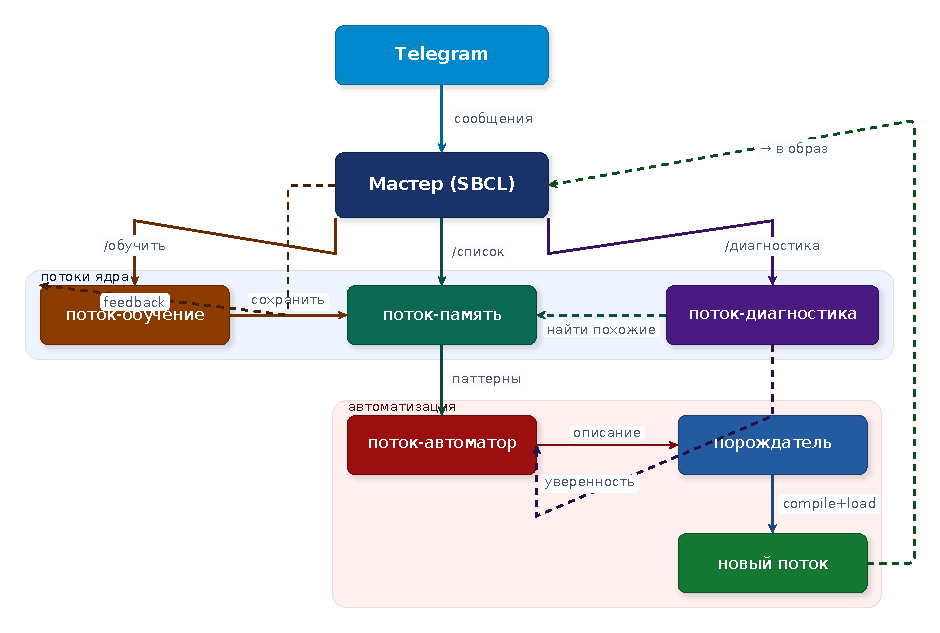
\includegraphics[width=0.88\textwidth]{arch_diagram.pdf}
  \caption{Архитектура саморазвивающегося потока}
\end{figure}

\subsection{Поток \texttt{память}}

\textbf{Назначение:} долговременное хранилище пар (проблема $\to$ решение) с поиском по сходству.

\textbf{Интерфейс:}
\begin{lstlisting}[language={},numbers=none]
/запустить память добавить: проблема=N+1 в GeoDjango | решение=select_related
/запустить память найти: медленный queryset с Point
/запустить память список
/запустить память удалить: 3
\end{lstlisting}

\textbf{Формат хранения} --- JSON:

\begin{lstlisting}[language=JSON,caption={Структура файла памяти}]
{
  "версия": 1,
  "примеры": [
    {
      "id": 1,
      "проблема": "N+1 запросы в GeoDjango при обходе связанных объектов",
      "решение": "select_related для FK, prefetch_related для M2M",
      "теги": ["django", "geodjango", "n+1"],
      "дата": "2026-03-14",
      "оценка": 1,
      "применений": 3,
      "паттерн": "orm-n+1"
    }
  ],
  "паттерны": {
    "orm-n+1": {
      "название": "N+1 оптимизация в Django ORM",
      "случаев": 5,
      "успешность": 1.0,
      "автоматизирован": true,
      "поток": "оптимизатор-orm"
    }
  }
}
\end{lstlisting}

\textbf{Три стратегии поиска} (по возрастанию качества/стоимости):

\begin{center}
\begin{tabular}{clll}
  \toprule
  \textbf{\#} & \textbf{Стратегия} & \textbf{Качество} & \textbf{Стоимость} \\
  \midrule
  1 & Keyword matching & Низкое & Бесплатно \\
  2 & LLM-сравнение & Среднее & Токены \\
  3 & Embedding + cosine & Высокое & API + модель \\
  \bottomrule
\end{tabular}
\end{center}

\textit{Рекомендация для MVP:} стратегия~2 (LLM-сравнение) --- оптимальный
баланс простоты и качества.

\subsection{Поток \texttt{обучение}}

\textbf{Назначение:} принимает новую пару от пользователя, валидирует, сохраняет в память, анализирует паттерн.

\textbf{Входной формат:}
\begin{lstlisting}[language={},numbers=none]
проблема: N+1 запросов при обходе Route.objects.all() с доступом к waypoints
решение: Route.objects.prefetch_related('waypoints')
теги: django, n+1, prefetch
\end{lstlisting}

\textbf{Логика обработки:}
\begin{enumerate}[leftmargin=1.5em]
  \item Парсинг входа (проблема, решение, теги)
  \item Проверка на дубликаты через \texttt{поток-память}
  \item Если похожая проблема уже есть --- предложить обновить или добавить как вариант
  \item Сохранение
  \item Анализ паттерна: «Это новый паттерн или вариация существующего?»
\end{enumerate}

\subsection{Поток \texttt{диагностика}}

\textbf{Назначение:} при новой проблеме ищет похожие, оценивает применимость, предлагает решение с уверенностью.

\textbf{Логика генерации решения:}

\begin{lstlisting}[language={},numbers=none,caption={Структура промпта диагностики}]
Найдены похожие проблемы и решения:

1. Проблема: <похожая 1>
   Решение: <решение 1>

2. Проблема: <похожая 2>
   Решение: <решение 2>

Новая проблема: <текст>

Предложи решение. После него укажи:
РЕШЕНИЕ: ...
УВЕРЕННОСТЬ: <0-100>
ОБОСНОВАНИЕ: ...
\end{lstlisting}

\textbf{Интерпретация уверенности:}

\begin{center}
\begin{tabular}{cll}
  \toprule
  \textbf{Диапазон} & \textbf{Статус} & \textbf{Действие} \\
  \midrule
  85--100\% & Высокая & Можно автоматизировать \\
  70--84\%  & Хорошая & Рекомендуется попробовать \\
  50--69\%  & Средняя & Проверить внимательно \\
  0--49\%   & Низкая  & Только гипотеза \\
  \bottomrule
\end{tabular}
\end{center}

\subsection{Поток \texttt{автоматор}}

\textbf{Назначение:} мониторинг паттернов и порождение специализированных потоков при достижении порогов.

\textbf{Пороги автоматизации:}

\begin{lstlisting}[language=CommonLisp,caption={Параметры порогов в Common Lisp}]
(defparameter *пороги*
  '((:предложение   . 30)    ; минимум для вывода предложения
    (:применение    . 70)    ; автоматическое применение с подтверждением
    (:автоматизация . 85)))  ; порождение нового потока
\end{lstlisting}

\textbf{Триггеры автоматизации:}
\begin{itemize}[leftmargin=1.5em]
  \item Уверенность $\geq 85\%$
  \item Паттерн встречался $\geq 3$ раз
  \item Пользователь подтверждал решение $\geq 2$ раз
\end{itemize}

% ═══════════════════════════════════════════════════════════════════
\section{Пример end-to-end}

\subsection{Сценарий из жизни GeoDjango разработчика}

\subsubsection{День 1 --- обучение}

\begin{lstlisting}[language={},numbers=none]
> /обучить
проблема: N+1 запросов при обходе Region.objects.all()
          с доступом к region.city
решение: Region.objects.select_related('city') -- один JOIN
теги: django, n+1, select_related

< Сохранено (id=1). Новый паттерн.
\end{lstlisting}

\subsubsection{День 3 --- ещё обучение}

\begin{lstlisting}[language={},numbers=none]
> /обучить
проблема: Медленная загрузка Point с prefetch связанных Polygon
решение: Point.objects.prefetch_related('polygons').only('id','geom')
теги: geodjango, prefetch

< Сохранено (id=2). Частичное сходство с id=1.
  Формируется паттерн: "Оптимизация ORM запросов"
\end{lstlisting}

\subsubsection{День 7 --- диагностика}

\begin{lstlisting}[language={},numbers=none]
> /диагностика Route.objects.all() с обходом route.waypoints.all()

< Найдено 2 похожих проблемы:

  1. (90%) N+1 при обходе Region с city
  2. (75%) Медленная загрузка Point с prefetch Polygon

  РЕШЕНИЕ: Route.objects.prefetch_related('waypoints')
  УВЕРЕННОСТЬ: 87%
  -- классический N+1, prefetch загрузит все waypoints одним запросом

  Применить? [да/нет]

> да

< Успешно. Паттерн "orm-n+1": 3 случая, 100% успешность.
  Рассматриваю автоматизацию...
\end{lstlisting}

\subsubsection{День 10 --- автоматизация}

\begin{lstlisting}[language={},numbers=none]
< Обнаружен устойчивый паттерн: "N+1 оптимизация в Django ORM"
  Случаев: 5, успешность: 100%, средняя уверенность: 89%

  Предлагаю создать поток «оптимизатор-orm».

  Создать? [да/нет]

> да

< Поток «оптимизатор-orm» порождён и загружен в образ.
  /запустить оптимизатор-orm "описание медленного queryset"
\end{lstlisting}

\begin{successbox}[title={Результат}]
За 10 дней система прошла путь от нуля до специализированного
автоматического потока, требующего минимального участия человека.
\end{successbox}

% ═══════════════════════════════════════════════════════════════════
\section{Реализация}

\subsection{Поток \texttt{память} (скелет)}

\begin{lstlisting}[language=CommonLisp,caption={поток-память.lisp --- ключевые функции}]
(defpackage :поток-память
  (:use :cl)
  (:export #:выполнить #:добавить-пример
           #:найти-похожие #:получить-все
           #:удалить-пример #:обновить-оценку))

(in-package :поток-память)

(defparameter *путь-памяти*
  (merge-pathnames "память.json" (user-homedir-pathname)))

;;; LLM-сравнение двух проблем
(defun похожи-p (проблема-1 проблема-2)
  "Возвращает :да, :частично или :нет"
  (let* ((промпт (format nil "Проблема А: ~A~%Проблема Б: ~A~%~
                              Похожи? Ответь: да, частично, нет"
                         проблема-1 проблема-2))
         (ответ (string-downcase (llm-запрос промпт))))
    (cond ((search "да" ответ)       :да)
          ((search "частично" ответ) :частично)
          (t                         :нет))))

;;; Поиск k ближайших
(defun найти-похожие (проблема &key (k 3))
  (let* ((с-оценками
          (mapcar (lambda (п)
                    (cons (похожи-p проблема
                                   (cdr (assoc :проблема п)))
                          п))
                  (примеры)))
         (отсортированы
          (sort с-оценками
                (lambda (a b)
                  (> (case (car a) (:да 2) (:частично 1) (t 0))
                     (case (car b) (:да 2) (:частично 1) (t 0)))))))
    (remove-if (lambda (x) (eq (car x) :нет))
               (subseq отсортированы 0 (min k (length отсортированы))))))

;;; Точка входа потока
(defun выполнить (задача)
  (handler-case
      (let ((команда (парсить-команду задача)))
        (case (first команда)
          (:добавить (format nil "Сохранено (id=~A)"
                             (добавить-пример (second команда)
                                              (third команда))))
          (:найти    (форматировать-результаты
                      (найти-похожие (second команда))))
          (:список   (форматировать-список (получить-все)))
          (:удалить  (удалить-пример (second команда)))))
    (error (e) (format nil "Ошибка: ~A" e))))
\end{lstlisting}

\subsection{Поток \texttt{диагностика} (ключевая логика)}

\begin{lstlisting}[language=CommonLisp,caption={Двухэтапная диагностика с self-critique}]
(defun диагностика-с-критикой (проблема)
  "Генерирует решение и критически его оценивает."
  (let* ((похожие (поток-память:найти-похожие проблема :k 5))
         (первичное (сгенерировать-решение проблема похожие))
         (критика
          (llm-запрос
           (format nil "Решение: ~A~%Проблема: ~A~%~
                        Критически оцени:~%~
                        1. Точно ли решает проблему?~%~
                        2. Побочные эффекты?~%~
                        3. Нужны уточнения?"
                   первичное проблема))))
    (format nil "~A~%~%Самопроверка:~%~A"
            первичное критика)))

(defun извлечь-уверенность (ответ)
  "Парсит УВЕРЕННОСТЬ: <N> из ответа LLM."
  (let ((поз (search "УВЕРЕННОСТЬ:" (string-upcase ответ))))
    (if поз
        (parse-integer
         (remove-if-not #'digit-char-p
                        (subseq ответ (+ поз 12) (+ поз 15))))
        50)))
\end{lstlisting}

\subsection{Поток \texttt{автоматор} (триггер и порождение)}

\begin{lstlisting}[language=CommonLisp,caption={Анализ готовности паттерна к автоматизации}]
(defparameter *мин-случаев*    3)
(defparameter *мин-успешность* 0.8)

(defun готов-к-автоматизации-p (статистика)
  (and (>= (getf статистика :случаев)    *мин-случаев*)
       (>= (getf статистика :успешность) *мин-успешность*)
       (>= (getf статистика :применений)
           (* 2 (getf статистика :случаев)))))

(defun породить-специализированный (статистика)
  (let ((описание (format nil
    "Создай поток ~A-оптимизатор.~%~
     Задача: принять описание проблемы и вернуть решение.~%~
     Паттерны проблема->решение:~%~{- ~A -> ~A~%~}"
    (getf статистика :название)
    (mapcan (lambda (п)
              (list (cdr (assoc :проблема п))
                    (cdr (assoc :решение п))))
            (subseq (getf статистика :примеры) 0 5)))))
    (поток-порождатель:выполнить описание)))
\end{lstlisting}

% ═══════════════════════════════════════════════════════════════════
\section{Эволюция и обратная связь}

\subsection{Жизненный цикл}

\begin{center}
\begin{tabular}{clp{6.5cm}}
  \toprule
  \textbf{Этап} & \textbf{Примеров} & \textbf{Поведение системы} \\
  \midrule
  Накопление    & $< 3$   & Сохраняет примеры, не предлагает решений \\
  Имитация      & $3-10$  & Few-shot промпт, решения с уверенностью \\
  Обобщение     & $10+$   & Выделяет абстрактные паттерны \\
  Автоматизация & $\geq3$ + критерии & Порождает специализированный поток \\
  \bottomrule
\end{tabular}
\end{center}

\subsection{Механизм обратной связи}

\begin{lstlisting}[language={},numbers=none]
/хорошо 5         -- пример id=5 помог, +1 к оценке
/плохо 5 "не то"  -- id=5 не подошёл, -1 + сохранить как антипаттерн
\end{lstlisting}

Антипаттерн сохраняется с префиксом «НЕ ДЕЛАТЬ:» и влияет на
future-диагностику --- система учится избегать неправильных решений.

\subsection{Защита от деградации}

\begin{enumerate}[leftmargin=1.5em]
  \item \textbf{Decay} --- влияние примеров без применений за 30+ дней постепенно снижается
  \item \textbf{Порог применений} --- минимум 2 успешных применения до участия в автоматизации
  \item \textbf{Self-critique} --- LLM оценивает паттерн перед порождением потока
  \item \textbf{Карантин} --- новые потоки первые 5 вызовов работают в режиме «предложение», не «применение»
\end{enumerate}

% ═══════════════════════════════════════════════════════════════════
\section{Roadmap}

\subsection{День 1 --- Минимальный MVP}

\begin{itemize}[leftmargin=1.5em]
  \item[\checkmark] \texttt{поток-память.lisp} с keyword matching (без LLM)
  \item[\checkmark] Добавление примеров, поиск, список
  \item[\checkmark] Тест: 3 примера + поиск похожего
\end{itemize}

\begin{lstlisting}[language=CommonLisp,caption={Поиск по словам без LLM для быстрого старта}]
(defun найти-по-словам (проблема примеры)
  (let ((слова (uiop:split-string (string-downcase проблема))))
    (sort примеры #'>
          :key (lambda (п)
                 (count-if (lambda (с)
                             (search с (string-downcase
                                        (cdr (assoc :проблема п)))))
                           слова)))))
\end{lstlisting}

\subsection{Неделя 1 --- Полный цикл имитации}

\begin{itemize}[leftmargin=1.5em]
  \item LLM-поиск по сходству в \texttt{поток-память}
  \item \texttt{поток-обучение} с валидацией дубликатов
  \item \texttt{поток-диагностика} с уверенностью
  \item Feedback (\texttt{/хорошо}, \texttt{/плохо})
\end{itemize}

\subsection{Неделя 2 --- Автоматизация}

\begin{itemize}[leftmargin=1.5em]
  \item \texttt{поток-автоматор} с порогами
  \item Интеграция с \texttt{порождатель}
  \item Карантин для новых потоков
  \item Тест полного цикла end-to-end
\end{itemize}

\subsection{Месяц 1 --- Production}

\begin{itemize}[leftmargin=1.5em]
  \item Self-critique, decay устаревших примеров
  \item UI для просмотра и редактирования памяти
  \item Экспорт / импорт, статистика
\end{itemize}

\subsection{Долгосрочно}

\begin{itemize}[leftmargin=1.5em]
  \item Embedding-based поиск (локальная модель или API)
  \item Иерархия паттернов (мета-паттерны)
  \item Интеграция с IDE через LSP extension
\end{itemize}

% ═══════════════════════════════════════════════════════════════════
\section{Риски и ограничения}

\begin{center}
\begin{tabularx}{\textwidth}{lLl}
  \toprule
  \textbf{Риск} & \textbf{Описание} & \textbf{Митигация} \\
  \midrule
  Контекстное окно
    & При 100+ примерах невозможно включить все в промпт
    & Жёсткий лимит: топ-5; batch-сравнение \\
  Drift качества
    & Устаревшие паттерны деградируют
    & Decay, тегирование версий \\
  Overfitting
    & Система учится неоптимальному стилю
    & Self-critique + флаг «проверено» \\
  Безопасность
    & Порождённый код может быть опасен
    & Sandboxing, timeout, карантин \\
  Стоимость LLM
    & N запросов на каждый поиск
    & Batch, кэш, дешёвая модель для сравнения \\
  \bottomrule
\end{tabularx}
\end{center}

\subsection{Стоимость LLM-запросов}

При 100 примерах и batch-сравнении:
$100 \times 5 \text{ токенов} \approx 500 \text{ токенов} \approx \$0.001$ за один поиск.
Приемлемо для персонального использования.

% ═══════════════════════════════════════════════════════════════════
\section{Заключение}

\subsection{Ключевые выводы}

\begin{enumerate}[leftmargin=1.5em]
  \item \textbf{In-context learning достаточен.} Fine-tuning избыточен и
    создаёт больше проблем (catastrophic forgetting, инфраструктура), чем решает.

  \item \textbf{Метациркулярность --- главное преимущество.} Порождатель уже
    существует в системе; саморазвивающийся поток --- его естественное расширение.

  \item \textbf{Gradual autonomy.} Переход от имитации к автоматизации
    должен быть постепенным, с явными checkpoint'ами: feedback, пороги, карантин.

  \item \textbf{Human-in-the-loop критичен.} Без обратной связи система
    неизбежно деградирует. Feedback --- не опция, а архитектурное требование.
\end{enumerate}

\subsection{Критерий успеха}

\begin{successbox}[title={Через месяц система считается успешной, если:}]
\begin{itemize}[leftmargin=1em]
  \item Инженер тратит меньше времени на повторяющиеся проблемы
  \item Есть $\geq 1$ автоматически порождённого полезного потока
  \item Точность предложений $> 70\%$
\end{itemize}
\end{successbox}

\subsection{Следующие шаги}

\begin{enumerate}[leftmargin=1.5em]
  \item Скопировать скелеты потоков (раздел~5) в \texttt{мастер/потоки/}
  \item Добавить 5 реальных примеров из GeoDjango-практики
  \item Использовать, давать feedback, наблюдать за эволюцией
\end{enumerate}

\vspace{1cm}
\hrule
\vspace{4mm}
{\small\color{MidGray}
  Документ подготовлен для Артемия.
  Версия~1.0, 14~марта~2026.
  Проект: \texttt{development\_system}.
}

\end{document}
